
\documentclass[a4paper, 12pt]{article}
\usepackage{graphicx}
\title{Exercise 1, Group 2 \\ TDT4258 \\ Energy Efficient Computer Systems}
\author{Per Bachmann \and Imre Kerr \and Kristian Volden}
\begin{document}
\maketitle
\begin{abstract}
	In this report, we describe and discuss the first exercise in the Energy efficient computer systems course. In this excercise we developed a simple program for an EFM32 Giant Gecko microcontroller. The program lets the user manipulate a row of LEDs (light emitting diodes) using buttons on a game pad. Low energy modes and interrupts are used to reduce power consumption.
\end{abstract}
\pagebreak
\section{Introduction} % (fold)
\label{sec:introduction}
	A microcontroller is a CPU with the most necessary components included on the same silicon die, i.e. the flexible GPIO I/O controller. The purpose of this integration is to allow for more minimal and energy efficient designs. The GPIO controller is included in the EFM32GG microcontroller and is essential for this exercise.
	
	An important aspect of this exercise is to use interrupts for controlling the buttons on the game pad. An interrupt, in contrast to continuously polling the I/O, allows the CPU to enter a low power state if there is no work to be done. The interrupt will then awake the CPU and start the necessary interrupt handler routine.
	
	For the exercise we were given access to an EFM32GG-DK3750 development board with an ARM Cortex M3 based EFM32GG microcontroller. We were also given access to a custom peripheral game pad, with buttons and LEDs, for the development board. For this microcontroller, we were expected to write a small program in the assembly programming language. The program should allow a user to use the buttons on the game pad to control the LEDs. The program should do this while using as little energy as possible.
% section introduction (end)

\section{Description and Methodology} % (fold)
\label{sec:description_and_methodology}
    \subsection{Description of the Program} % (fold)
    \label{sub:description_of_program}
        The functionality of the program is very simple. A single LED will be lit on the gamepad, and the user can press button 1 and 3 (``left'' and ``right'') to move the light left or right.

        A few things must be set up before the main program logic can begin. This is all included in the compendium, but is duplicated here for completeness.

        \begin{enumerate}
            \item Enable GPIO clock in CMU.
            \item Enable interrupts from the GPIO (both even and odd pins).
            \item Set port A pin 8-15 (the LEDs) as output with high drive strength.
            \item Set port C pin 0-7 (the buttons) as input with glitch filter.
            \item Enable pull-up resistors for port C pin 0-7.
            \item Enter sleep mode.
        \end{enumerate}

        Before entering sleep mode, the value \texttt{0xFEFEFEFE} is written to a register and then to port A output. This corresponds to one LED being turned on. From then on, the GPIO interrupt handler will detect if button 1 or 3 has been pressed. If so, the handler rotates this value one position in the appropriate direction and writes it to the data out register. Since we want to rotate with a period of 8, but the registers are 32 bits, we duplicate the output value four times.

        In the interrupt handler, we must clear the GPIO interrupt flag register by writing \texttt{0xFF} to \texttt{GPIO\_IFC}. We found that this has to happen at the start of the handler, otherwise a second interrupt could be triggered while the handler is running.
    % subsection description_of_program (end)

    \subsection{Methodology} % (fold)
    \label{sub:methodology}
        Our methodology was as follows:
        \begin{enumerate}
            \item Get the hardware and uploading working (Exercise 0).
            \item Write a program that turns on some LEDs.
            \item Modify it to use buttons as well. This version used a busy loop to constantly write the button state to the LEDs.
            \item Modify it to do the same thing, only with interrupts.
            \item Write the final functionality for the program. Having gotten GPIO and interrupts working, this step was easy once we remembered how boolean logic works.
            \item Test the program and fix any problems.
        \end{enumerate}
    % subsection methodology (end)
% section description_and_methodology (end)

\section{Results and Tests} % (fold)
\label{sec:results_and_tests}
	\subsection{Functional Tests} % (fold)
	\label{sub:functional_tests}
        \begin{figure}[!ht]
        \centerline{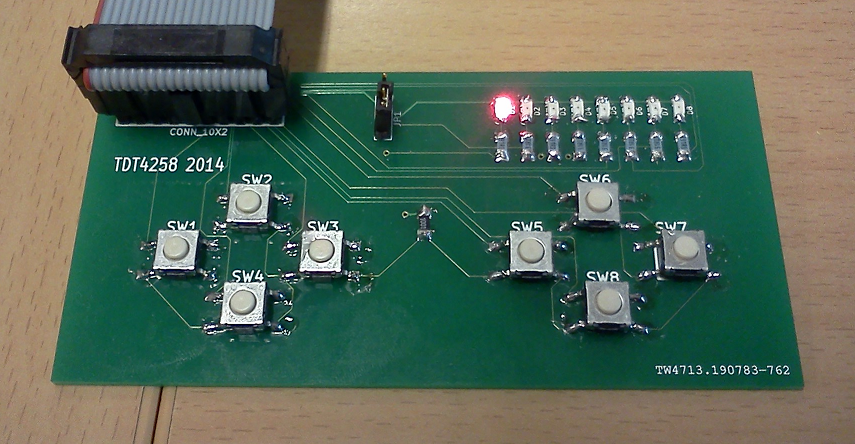
\includegraphics[width=0.7\textwidth]{IMG064}}
        \centerline{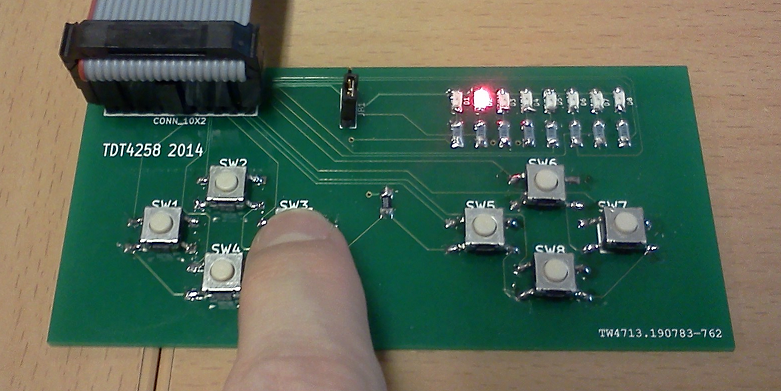
\includegraphics[width=0.7\textwidth]{IMG065}}
        \caption{Pressing the buttons makes the light move.}
        \label{fig:buttons}
        \end{figure}
		\begin{enumerate}
			\item Pressing the left (button 1) or right (button 3) buttons should make the light move left or right, respectively. \\
				  Result: It does.
			\item The buttons should not glitch, i.e. a press should not be registered twice.\\
				  Result: This did happen occasionally.
		\end{enumerate}
		For the last one, our theory is that the built-in glitch filter in the EFM32GG has a period that is too short (10-50ns according to the data sheet). Since it is implemented in hardware, this period isn't user configurable.
	% subsection functional_tests (end)

	\subsection{Power Consumption} % (fold)
	\label{sub:power_consumption}
		\begin{figure}[!ht]
        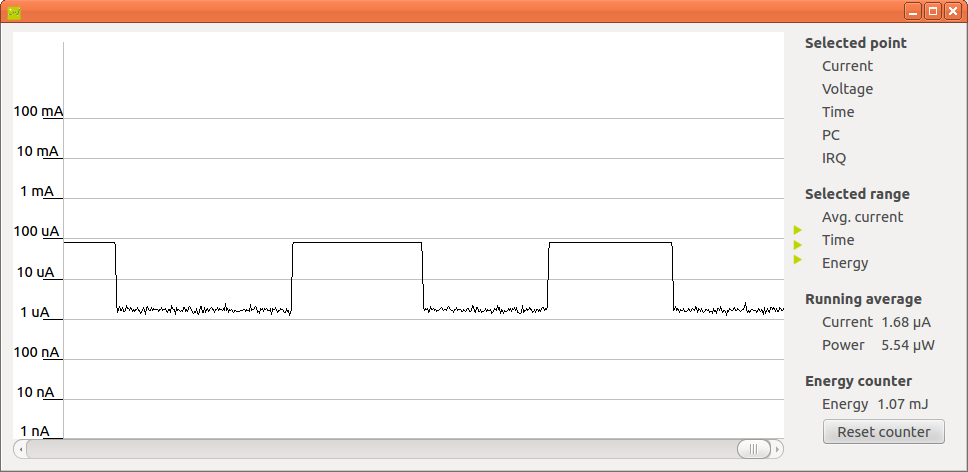
\includegraphics[width=\textwidth]{eaprofiler}
        \caption{eaProfiler graph showing power consumption}
        \label{fig:profiler}
        \end{figure}
        The graph in Figure \ref{fig:profiler} shows the difference in power consumption for one button pressed and no buttons pressed. When no buttons are pressed, the power consumption is very low, only 5.54 $\mu$W. When a button is pressed, the power consumption increases considerably. Note that this is due to current flowing through the switch to ground, not because the MCU is running all the time.

        Also note that the LED is not included in the calculation, because it would dwarf everything else.
	% subsection power_consumption (end)
% section results_and_tests (end)

\section{Evaluation of Assignment} % (fold)
\label{sec:evaluation_of_assignment}
	The assignment was a good introduction to using the EFM32GG microcontroller. The compendium was easy to follow and made the task manageable. However the use of the reference manual was tedious, as it was not always easy to look up the information you actually needed. As an example we tried to find out how to return from the interrupt handler; looking at the quick reference and tried to find the instruction there, but were unable to do so. You may be able to find it in the 900 page reference manual, but trying to search through the manual for a task like this should not be necessary. Even though you want us to look at the reference manual, it should be for those things that we could realistically be expected to find there. Other than this, the exercise served as a good introduction to the course.
% section evaluation_of_assignment (end)

\section{Conclusion} % (fold)
\label{sec:conclusion}
    In this assignment, we have learned several important techniques for energy efficient computer system development. We have seen that interrupts and energy modes are vital to keeping power usage low. The exercise also served as a gentle introduction to low-level programming which is quite different from the programming we are used to. While the rest of the exercises won't use assembly language, knowledge of very low level programming can be useful in the real world, especially for real-time systems.
% section conclusion (end)

\section{References} % (fold)
\label{sec:references}
    \begin{itemize}
        \item TDT4258 Exercise Compendium, from the course pages on It's Learning.
        \item ARM Thumb-2 Quick Reference, from the course pages on It's Learning.
        \item EFM32GG990 Datasheet, \\
		\textit{http://cdn.energymicro.com/dl/devices/pdf/d0046\_efm32gg990\_datasheet.pdf}
    \end{itemize}
% section references (end)
\end{document}